\begin{figure}[t]
	\center
	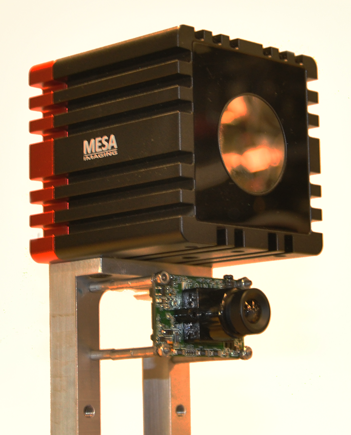
\includegraphics[width = 5cm]{camerasetup.png}
	\caption[SwissRanger depth camera and Firefly color camera setup]{SwissRanger depth 
		camera (top) and Firefly color camera (bottom) setup.}
	\label{camerassetup}
\end{figure}

Figure \ref{camerassetup} shows a setup of two camera sensors fixed on a frame, one below the other. The 
camera at the bottom is a Firefly, a Firewire camera manufactured by Point Grey \cite{FireflyDatasheet}. 
It captures grayscale images that can be converted to color using functions from the libdc1394 library
(see Section \ref{dc1394javaacquire}). The size of the images captured by a Firefly is $640 \times 480$ 
pixels.

The camera on top is a SwissRanger SR4000, a 3D time-of-flight camera manufactured by Mesa Imaging. 
It captures x-coordinate, y-coordinate, and z-coordinate information from the scene 
in front of the camera. This chapter focuses on the z-coordinate data, which will be referred to from this point 
on as the \textit{depth image}.\footnote{Similarly, the SwissRanger camera will also be referred to as the 
\textit{depth camera}.} The SwissRanger also produces an amplitude image, which corresponds to 
the amplitude of the modulated signal used in the depth measurements. The amplitude image can be used 
both for generating a grayscale image representing the captured scene and for measuring the quality of the 
depth values \cite{SR4000Manual}. The size of all images captured by the SwissRanger is $176 \times 144$
pixels.

Depending on the lens in the Firefly, the field of view of the color camera can be inside the field of view of the 
SwissRanger, or vice versa. Since the Firefly is more flexible in the matter of changing its field of view, this 
setup uses a wide angle lens on the color camera that makes it encompass the field of view of the depth 
camera. Figure \ref{imagetypes} shows an example of the three types of images captured by this 
depth-color camera setup. 
 

\begin{figure}[t]
	\center
	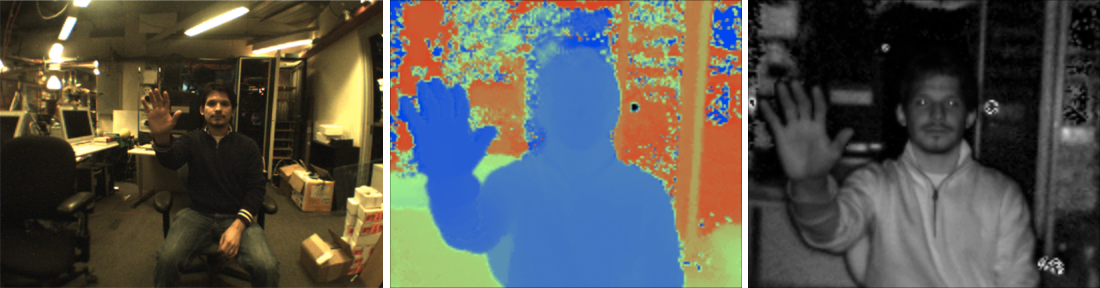
\includegraphics[width = 15cm]{data.png}
	\caption[Image types captured by the depth-color camera setup]{Image types captured by the 
		depth-color camera setup. From left to right: color image, depth image, and amplitude image.
		Notice the difference between the field of views of both cameras.}
	\label{imagetypes}
\end{figure}